\documentclass[a4paper]{ctexart}
\usepackage{amsmath, amsthm, amssymb, graphicx, wrapfig, enumitem, titlesec, geometry, mathtools, bm}
\usepackage{booktabs,array,float}

\geometry{left=2.5cm, right=2.5cm, top=3cm, bottom=3cm}
\setlength{\parindent}{0pt}

% === 技巧框定义 ===
\usepackage{tcolorbox}
\tcbuselibrary{skins, breakable}

\newtcolorbox{tipbox}{
  enhanced,
  breakable,
  colback=green!3!white,        % 浅绿背景
  colframe=teal!50!black,       % 墨绿色边框
  colbacktitle=teal!30!white,   % 标题背景
  coltitle=black,               % 标题颜色
  fonttitle=\bfseries\large,
  title=Tips,
  attach boxed title to top left={xshift=10mm, yshift=-3mm},
  boxed title style={size=small, colframe=teal!50!black},
  left=5mm, right=5mm, top=5mm, bottom=5mm,
  borderline west={3pt}{0pt}{teal!50!black},  % 左侧粗装饰线
  sharp corners=south,
  before skip=12pt,
  after skip=12pt,
}

\newtheorem{example}{例}[section] 
\renewcommand{\proofname}{\textbf{解:}}
\title{概率论考前复习}
\author{Drake Pan}
\date{Jun.2026}

\begin{document}
\maketitle
\newpage
\tableofcontents
\newpage

\section{随机事件与概率}

事件的互不相容：两个事件没有共同的样本点，即：
\begin{equation}
    A \cap B = \varnothing
\end{equation}
事件之间可以进行运算，$n$个事件之间进行交或者并的运算，当：
\begin{itemize}
    \item n为$\infty$，则称该运算是\textbf{可列的}。
    \item n为有限值，则称该运算是\textbf{有限的}。
\end{itemize}
\textbf{差运算}是一个常见运算，其定义是：
\begin{equation}
    A-B=A\overline{B}
\end{equation}
事件运算有以下的规律：
\begin{itemize}
    \item 交换律：交与并
    \item 结合律：交与并
    \item 分配律：交与并
    \item \textbf{De Morgan定律}（对偶律）
        \[
        \begin{aligned}
            \overline{A \cup B} &= \bar{A} \cap \bar{B} \\[6pt]
            \overline{A \cap B} &= \bar{A} \cup \bar{B}
        \end{aligned}
        \]
\end{itemize}
De Morgan定律还可以进行推广到$n$个有限的情形和可列的情形。
下面考虑概率，其满足可列可加性公理，即若$A_1\cdots A_n$都是互不相容的，那么：
\begin{equation}
    P(\cup_{i=1}^{\infty} A_i) = \sum_{i=1}^{\infty} P(A_i)
\end{equation}
注意，概率也满足有限可加性。
两个事件的差满足：
\begin{equation}
    P(A-B)=P(A)-P(AB)
\end{equation}
两个事件的并:
\begin{equation}
    P(A\cup B) = P(A)+P(B)-P(AB)
\end{equation}
推广到$n$个事件有：
\begin{equation}
    P\left(\bigcup_{i=1}^{n} A_i\right) = \sum_{ i=1}^{n} P(A_i) - \sum_{1 \leq i < j \leq n} P(A_i \cap A_j) + \sum_{1 \leq i < j < k \leq n} P(A_i \cap A_j \cap A_k) - \cdots + (-1)^{n-1} P\left(\bigcap_{i=1}^{n} A_i\right)
\end{equation}
一个常见的例子是配对问题：
\begin{example}
    在一个有$n$个人参加的晚会上，每个人带了一件礼物，且假定各人带的礼物都不相同。晚会期间各人从放在一起的$n$件礼物中随机抽取一件，问至少有一个人自己抽到自己礼物的概率是多少？
\end{example}
\begin{proof}
    一眼看上去貌似对立事件更为简单，实则不然。我们直接考虑原事件，尝试把这个时间拆分为若干个小事件的运算结果。

    设$A_i$为“第$i$个人拿到了自己的礼物，则$A=\cup_{i=1}^n A_i$，运用上述给出的公式，有：
    \begin{align*}
        P(A_1) &= P(A_2) = \cdots = P(A_n) = \frac{1}{n}, \\
        P(A_1A_2) &= P(A_1A_3) = \cdots = P(A_{n-1}A_n) = \frac{1}{n(n-1)}, \\
        P(A_1A_2A_3) &= P(A_1A_2A_4) = \cdots = P(A_{n-2}A_{n-1}A_n) = \frac{1}{n(n-1)(n-2)}, \\
        &\qquad \cdots \\
        P(A_1A_2\cdots A_n) &= \frac{1}{n!}.
    \end{align*}
    那么可以得到：
    \[ P(A) = 1 - \frac{1}{2!} + \frac{1}{3!} - \frac{1}{4!} + \cdots + (-1)^{n-1} \frac{1}{n!}. \]
\end{proof}
\begin{tipbox}
    放回抽样。若总体有$k$类，抽取$n$次，那么各类型出现次数服从多项分布。
\end{tipbox}
几何概率：任意一点落在区域中是等可能的，那么度量概率：
\begin{equation}
    P(A)=\dfrac{S_A}{S_{\Omega}}
\end{equation}
几个常见的例子是：
\begin{center}
    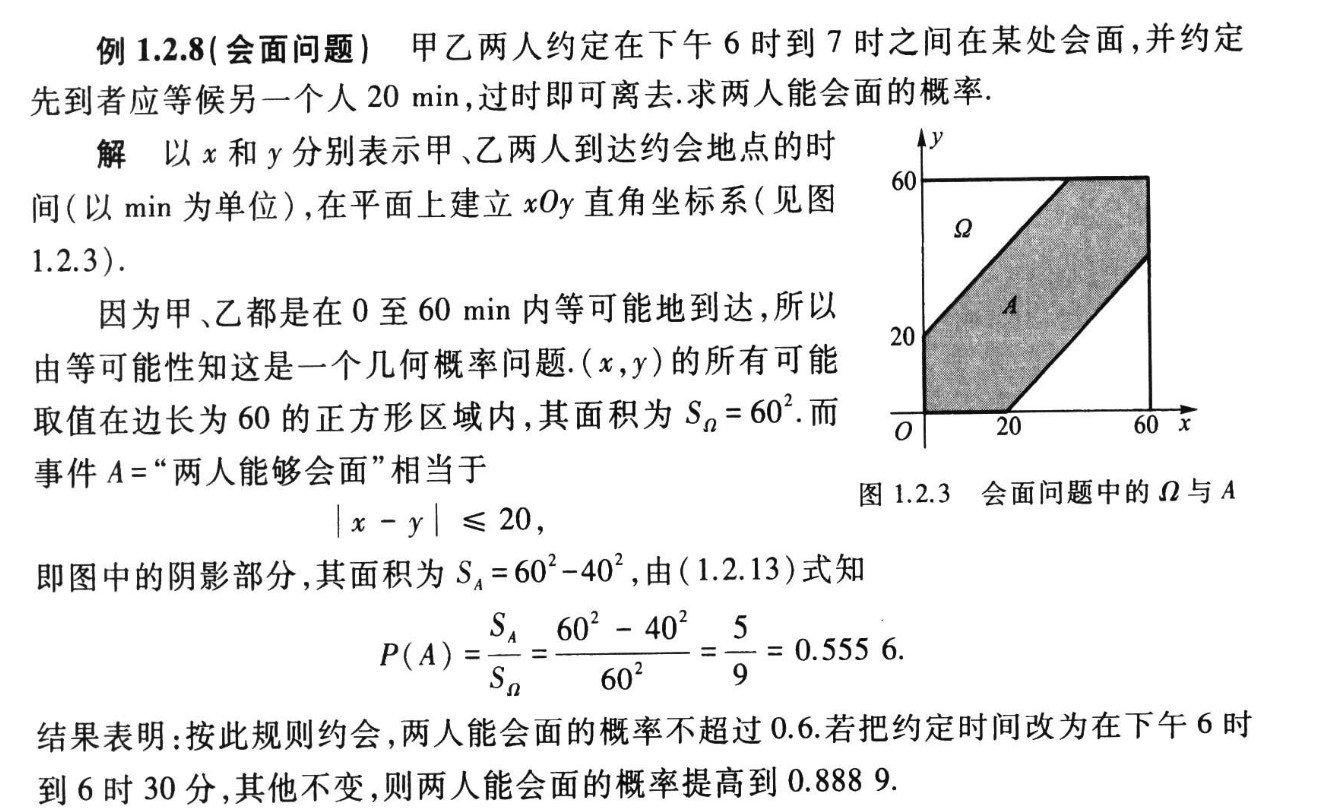
\includegraphics[width=0.8\textwidth]{1.jpg}
\end{center}
\begin{center}
    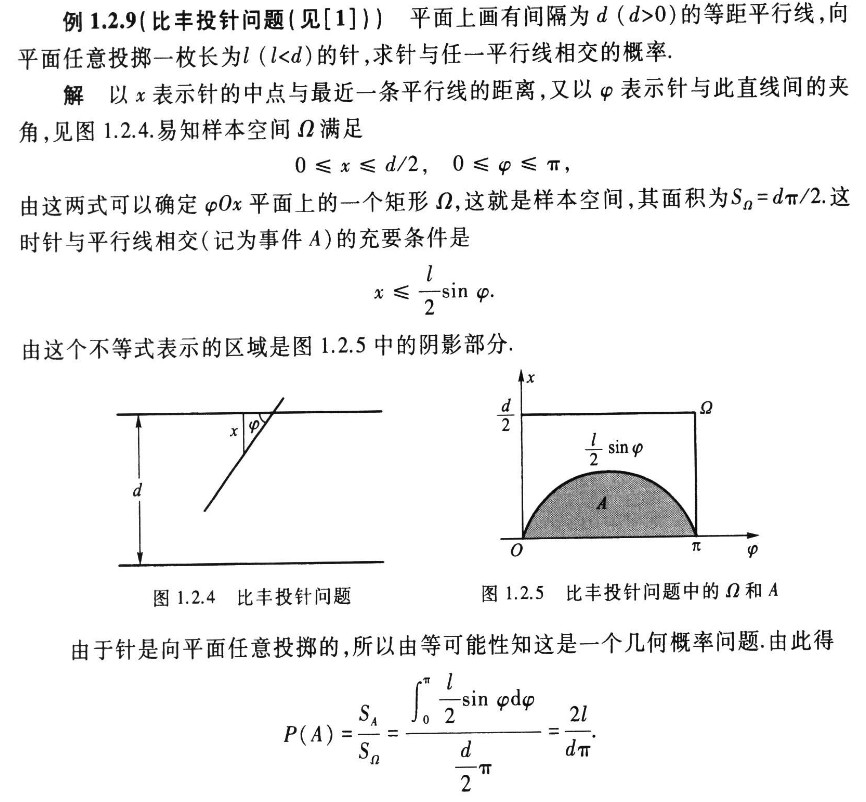
\includegraphics[width=0.8\textwidth]{2.jpg}
\end{center}
条件概率：
\begin{equation}
    P(A|B)=\dfrac{P(AB)}{P(B)}
\end{equation}
一个常见的例子是Pólya罐子模型：
\begin{example}
    一个罐子初始装有 \( a \) 个黑球和 \( b \) 个红球。现进行如下随机试验：每次从罐中随机取出一球，记录其颜色，然后将该球放回并额外加入 \( c \) 个同色球（\( c \) 为正整数）。重复这一过程。 \\
    (1) 求第二次抽到黑球的概率。 \\
    (2) 证明抽取结果序列具有可交换性。(即只要黑球和红球的出现次数相同，顺序不影响概率) \\
    (3) 令 \( X_n \) 为第 \( n \) 次抽取后黑球所占比例，证明 \( X_n \) 几乎必然收敛到某个随机变量 \( X \)，并指出 \( X \) 的分布。
\end{example}
\begin{proof}
    \textbf{(1) 第二次抽到黑球的概率}

    \begin{align*}
    P(B_2)&=P(B_1)P(B_2|B_1)+P(R_1)P(B_2|R_1)\\
    &=\frac{a}{a+b}\cdot\frac{a+c}{a+b+c}+\frac{b}{a+b}\cdot\frac{a}{a+b+c}\\
    &=\frac{a(a+c)+ab}{(a+b)(a+b+c)}=\frac{a(a+b+c)}{(a+b)(a+b+c)}=\frac{a}{a+b}.
    \end{align*}

    \textbf{(2) 可交换性证明}

    任意含$k$个黑、$n-k$个红的特定序列概率为
    \[
    \frac{a(a+c)\cdots(a+(k-1)c)\cdot b(b+c)\cdots(b+(n-k-1)c)}{(a+b)(a+b+c)\cdots(a+b+(n-1)c)},
    \]
    仅与$k$有关，与顺序无关，故可交换。

    \textbf{(3) 极限分布}(直观理解)

    \begin{enumerate}
        \item 波利亚罐等价于：先随机抽取 $U \sim \text{Beta}(a/c, b/c)$，然后独立地以概率 $U$ 抽黑球。
        \item 此时黑球比例 $X_n$ 收敛到 $U$。
        \item 因此 $X = U \sim \text{Beta}(a/c, b/c)$。
    \end{enumerate}
\end{proof}
此基础上还衍生出了计算后验概率的Bayes公式：设 $A_1, A_2, \ldots, A_n$ 为样本空间的一个完备事件组（即两两互斥且并集为全集），$P(A_i) > 0$，$B$ 为任意事件且 $P(B) > 0$，则
\begin{equation}
    P(A_i \mid B) = \frac{P(B \mid A_i) P(A_i)}{\sum_{j=1}^{n} P(B \mid A_j) P(A_j)}
\end{equation}
最后，两个事件独立定义为：
\begin{equation}
    P(AB)=P(A)P(B)
\end{equation}
这个概念要与互不相容做出清晰的区分。
\begin{tipbox}
    零概率事件不一定是不可能事件。比如飞镖扎在正方形中心概率为$0$（点的面积是0），但并不代表他是不可能事件。
\end{tipbox}
在解题过程中，常会涉及一些方法，比如数学归纳法：
\begin{example}
    设罐中有 \( b \) 个黑球、\( r \) 个红球，每次随机取出一个球，取出后将原球放回，再加入 \( c \) (\( c > 0 \)) 个同色的球。试证：第 \( k \) 次取到黑球的概率为 \( b/(b+r) \)，\( k = 1, 2, \dots \)。
\end{example}

\begin{proof}
    设事件 \( A_i(b,r) \) 为“罐中有 \( b \) 个黑球、\( r \) 个红球时，第 \( i \) 次取到的是黑球”，记
    \[ p_i(b,r) = P(A_i(b,r)), \quad i = 1, 2, \dots \]
    则显然有
    \[ p_1(b,r) = b/(b+r). \]
    下用归纳法证明。

    设 $p_{k-1}(b,r) = b/(b+r)$
    则由全概率公式得
    \begin{align*}
        p_k(b,r) &= P(A_k(b,r)) \\
        &= P(A_1(b,r)) P(A_k(b,r) \mid A_1(b,r)) \\
        &\quad + P(\overline{A_1}(b,r)) P(A_k(b,r) \mid \overline{A_1}(b,r)).
    \end{align*}

    我们把 \( k \) 次取球分为两段：第 1 次取球与后 \( k-1 \) 次取球。当第 1 次取到黑球时，罐中增加 \( c \) 个黑球，这时从原罐中第 \( k \) 次取到黑球等价于从新罐（含 \( b+c \) 个黑球，\( r \) 个红球）中第 \( k-1 \) 次取到黑球，故有
    \[ P(A_k(b,r) \mid A_1(b,r)) = P(A_{k-1}(b+c, r)) = \frac{b+c}{b+r+c}, \]
    类似有
    \[ P(A_k(b,r) \mid \overline{A_1}(b,r)) = P(A_{k-1}(b, r+c)) = \frac{b}{b+r+c}. \]

    代入上式得
    \[ p_k(b,r) = \frac{b}{b+r} \times \frac{b+c}{b+r+c} + \frac{r}{b+r} \times \frac{b}{b+r+c} = \frac{b}{b+r}. \]
    由归纳法知结论成立。
    （此处不用前$k-1$次和最后一次，是因为前$k-1$次取完之后罐子中的球状态数量都是不确定的，因此没法用归纳假设。）
\end{proof}
还有投掷硬币的经典问题：
\begin{example}
    甲掷硬币 \( n + 2 \) 次，乙掷 \( n \) 次，求甲掷出的正面数比乙掷出的正面数多的概率。
\end{example}

\begin{proof}
    记 \( A = \) 甲掷出的正面数 > 乙掷出的正面数，  
        \( B = \) 甲掷出的反面数 > 乙掷出的反面数。

    由对称性知：\( P(A) = P(B) \)，又因为 \( A \cap B = \emptyset \)，所以 \( A \cup B = \Omega \)。

    由此得
    \[
    1 = P(A \cup B) = P(A) + P(B) - P(AB). \tag{1}
    \]

    注意到 \( AB \neq \emptyset \)，且
    \[
    \begin{aligned}
    AB &= \text{甲的正面数 > 乙的正面数，甲的反面数 > 乙的反面数} \\
    &= \text{甲的正面数 - 乙的正面数 = 1，甲的反面数 - 乙的反面数 = 1} \\
    &= \text{甲的正面数 - 乙的正面数 = 1}.
    \end{aligned}
    \]

    所以有
    \[
    \begin{aligned}
    P(AB) &= \sum_{i=0}^n P(\text{甲的正面数} = i + 1,\ \text{乙的正面数} = i) \\
    &= \sum_{i=0}^n \binom{n+2}{i+1} \binom{n}{i} \left( \frac{1}{2} \right)^{2n+2} \\
    &= \frac{1}{2^{2n+2}} \sum_{i=0}^n \binom{n+2}{i+1} \binom{n}{i} \\
    &= \frac{1}{2^{2n+2}} \binom{2n+2}{n+1}.
    \end{aligned}
    \]

    将此结果及 \( P(A) = P(B) \) 代入 (1) 式得
    \[
    P(A) = \frac{1}{2} \left[ 1 + \frac{1}{2^{2n+2}} \binom{2n+2}{n+1} \right].
    \]
    额外的讨论：如果假设甲投掷$n-1$次，那么改变的就是$AB$，此时$AB=\emptyset$，那么$P(A)=\dfrac{1}{2}$这是一个优美的经典结论。
\end{proof}
此外我们还经常使用递推方法：
\begin{example}
    甲、乙、丙三人进行比赛，规定每局两个人比赛，胜者与第三人比赛，依次循环，直至有一人连胜两次为止，此人即为冠军。而每次比赛双方取胜的概率都是 \(1/2\)，现假定甲、乙两人先比，试求各人得冠军的概率。
\end{example}
\begin{proof}
    我们假设如下三个概率：
    \begin{itemize}
        \item $p_1$：已经获胜了一场最终取胜的概率
        \item $p_2$：刚刚上场获胜的概率
        \item $p_3$：正在旁观的获胜概率
    \end{itemize}
    那么这三个概率会不断转化，有：
    \begin{equation*}
        \begin{aligned}
            p_1=\dfrac{1}{2}+\dfrac{1}{2} p_3\\
            p_2=\dfrac{1}{2}p_1+\dfrac{1}{2} p_3\\
            p_3=\dfrac{1}{2}p_2
        \end{aligned}
    \end{equation*}
    求解直接得到各个数值，那么有：$P_{\text{甲}}=P_{\text{乙}}=\dfrac{1}{2}(p_1+p_3)=\dfrac{5}{14},P_{\text{丙}}=p_2=\dfrac{2}{7}$
\end{proof}

\section{随机变量及其分布}

分布函数的连续性是右连续：
\begin{equation}
    \lim_{x\to x_0+0} F(x)=F(x_0)
\end{equation}
均值，方差的计算性质：
\begin{itemize}
    \item $E(A+B) = E(A) + E(B)$
    \item $E(aX) = aE(X)$
    \item $\operatorname{Var}(aX+b) = a^2 \operatorname{Var}(X)$
\end{itemize}
\begin{tipbox}  
    虽然这些性质是简单的，但是复杂问题的计算时往往是最重要的，一定要注意题目到底在对谁求方差，这对于判断到底谁是常数至关重要。
\end{tipbox}
Chebyshev不等式：描绘了随机变量关于期望的偏离，
\begin{equation}
    P(|X-E(X)|\geq \epsilon) \leq \dfrac{1}{\epsilon^2} Var(X) 
\end{equation}
下面来讨论各种常用的分布：分别是离散的和连续的，先来看离散分布。

\vspace{6pt}
    \begin{center}
        \begin{tabular}{|c|c|c|c|}
        \hline
        分布 & $P(X=k)$ & $E(X)$ & $\mathrm{Var}(X)$ \\
        \hline
        二项分布 $B(n,p)$ & $\dbinom{n}{k}p^k(1-p)^{n-k}$ & $np$ & $np(1-p)$ \\
        \hline
        泊松分布 $P(\lambda)$ & $\dfrac{\lambda^k e^{-\lambda}}{k!}$ & $\lambda$ & $\lambda$ \\
        \hline
        几何分布 Ge($p$) & $(1-p)^{k-1}p$ & $\dfrac{1}{p}$ & $\dfrac{1-p}{p^2}$ \\
        \hline
        负二项分布 Nb($r,p$)& $\dbinom{k-1}{r-1}p^r(1-p)^{k-r}$ & $\dfrac{r}{p}$ & $\dfrac{r(1-p)}{p^2}$ \\
        \hline
        \end{tabular}
        \end{center}

        \begin{tipbox}
            \begin{itemize}
                \item 二项分布取 $n=1$ 时成为两点分布，其概率函数可以写为：
                \[
                p(x) = p^x (1-p)^{1-x}, \quad x = 0, 1
                \]
                
                \item 若 $X_i \sim b(1, p)$，则
                \[
                \sum_{i=1}^n X_i \sim b(n, p)
                \]
                这种分布的可加性将在后面专门列出表格总结。
                
                \item 几何分布满足无记忆性质，即
                \[
                P(X > m + n \mid X > m) = P(X > n)
                \]
                
                \item 当 $n$ 很大、$p$ 很小，但 $np$ 值适中有限时，\textbf{二项分布可以用泊松分布做近似}。
                \[
                \binom{n}{k} p^k (1-p)^{n-k} \approx \frac{(np)^k e^{-np}}{k!}, \quad k = 0, 1, 2, \dots
                \]
            \end{itemize}
        \end{tipbox}
        下面再来看常用的连续分布：

        \vspace{6pt}
        \begin{center}
        \begin{tabular}{|c|c|c|c|}
        \hline
        \textbf{分布} & \textbf{概率密度函数 } $f(x)$ & \textbf{期望 } $E(X)$ & \textbf{方差 } $\mathrm{Var}(X)$ \\
        \hline
        正态分布 $N(\mu,\sigma^2)$ & $\dfrac{1}{\sigma\sqrt{2\pi}} e^{-\frac{(x-\mu)^2}{2\sigma^2}},\quad x\in\mathbb{R}$ & $\mu$ & $\sigma^2$ \\
        \hline
        均匀分布 $U(a,b)$ & $\dfrac{1}{b-a},\quad x\in[a,b]$ & $\dfrac{a+b}{2}$ & $\dfrac{(b-a)^2}{12}$ \\
        \hline
        指数分布 $\mathrm{Exp}(\lambda)$ & $\lambda e^{-\lambda x},\quad x\ge 0$ & $\dfrac{1}{\lambda}$ & $\dfrac{1}{\lambda^2}$ \\
        \hline
        伽马分布 $Ga(\alpha,\beta)$ & $\dfrac{\beta^\alpha}{\Gamma(\alpha)} x^{\alpha-1} e^{-\beta x},\quad x>0$ & $\dfrac{\alpha}{\beta}$ & $\dfrac{\alpha}{\beta^2}$ \\
        \hline
        贝塔分布 $\mathrm{Beta}(\alpha,\beta)$ & $\dfrac{x^{\alpha-1}(1-x)^{\beta-1}}{\mathrm{B}(\alpha,\beta)},\quad x\in[0,1]$ & $\dfrac{\alpha}{\alpha+\beta}$ & $\dfrac{\alpha\beta}{(\alpha+\beta)^2(\alpha+\beta+1)}$ \\
        \hline
        卡方分布 $\chi^2(n)$ & $\dfrac{x^{\frac{n}{2}-1} e^{-\frac{x}{2}}}{2^{\frac{n}{2}} \Gamma(\frac{n}{2})},\quad x>0$ & $n$ & $2n$ \\
        \hline
    \end{tabular}
\end{center}
\begin{tipbox}
    \begin{itemize}
        \item 正态分布$N(0,1)$称为标准正态分布，其CDF常用$\Phi(x)$表示：
        \[\Phi(x)=P(X\leq x)\]
        此数值往往通过查表获得，也是许多题目解的最终目标。对于一个任意正态分布，总可以通过如下的变量代换变为标准正态分布：
        \[
        X \sim N(\mu,\sigma^2) \quad \Rightarrow \quad Z = \frac{X-\mu}{\sigma} \sim N(0,1)
        \]
        此外，$\Phi(x)$还有常用性质 $\Phi(-x)=1-\Phi(x)$
        \item  指数分布是Gamma分布的特例：
        \[Exp(\lambda)=Ga(1,\lambda)\]
        其同样也是无记忆性的：
        \[P(X>s+t|X>s)=P(X>t)\]
        \item Gamma分布的定义来源于Gamma函数：
        \[
        \Gamma(\alpha) =\int_0^{\infty} x^{\alpha-1}e^{-x} dx
        \]
        \item Beta函数为:
        \[Beta(a,b)=\int_0 ^1 x^{a-1}(1-x)^{b-1} dx\]
        其与Gamma函数的关系是：
        \[Beta(a,b)=\dfrac{\Gamma(a)\Gamma(b)}{\Gamma(a+b)}\]
        \item $\chi^2(n)=Ga(\dfrac{n}{2},\dfrac{1}{2})$
    \end{itemize}
\end{tipbox}
当变换函数的自变量时，概率密度函数会发生如下变化：设 $X$ 为连续随机变量，密度函数为 $p_X(x)$。$Y = g(X)$ 连续，且 $g$ 严格单调，反函数 $h$ 有连续导数。则 $Y$ 的密度函数为
\begin{equation}
    p_Y(y) = p_X(h(y)) \cdot |h'(y)|, \quad a < y < b,
\end{equation}
当然这种方法可能会遇到一些困难，更普遍的办法时从CDF:$F_Y(y)=P(g(X)\leq y)$出发考虑，先求解CDF。
针对一些常见的分布，我们有些现成的结论：
\begin{itemize}
    \item \textbf{正态线性变换：} $X \sim N(\mu, \sigma^2) \Rightarrow Y = aX + b \sim N(a\mu + b,\ a^2\sigma^2),\ a \neq 0$。
    
    \item \textbf{伽马尺度变换：} $X \sim Ga(\alpha, \lambda) \Rightarrow Y = kX \sim Ga(\alpha,\ \lambda/k),\ k > 0$。
    \begin{itemize}
        \item 特例：$X \sim \chi^2(n) \Rightarrow Y = cX \sim Ga\left(\frac{n}{2},\ \frac{1}{2c}\right)$。
    \end{itemize}
    
    \item \textbf{概率积分变换：} 若 $F_X$ 严格单调连续，则 $Y = F_X(X) \sim U(0,1)$。
    \begin{itemize}
        \item 逆变换：若 $U \sim U(0,1)$，则 $F_X^{-1}(U) \sim X$（随机数生成基础）。
    \end{itemize}
    
    \item \textbf{指数与伽马关系：} 若 $X_1,\ldots,X_n$ 独立同分布于 $Exp(\lambda)$，则 $\sum_{i=1}^n X_i \sim Ga(n,\lambda)$。
    
    \item \textbf{卡方与正态关系：} 若 $Z_1,\ldots,Z_n$ 独立同分布于 $N(0,1)$，则 $\sum_{i=1}^n Z_i^2 \sim \chi^2(n)$。
    
\end{itemize}

\section{多维随机变量及其分布}
把上一章中的部分函数进行高维推广，可以得到一些常用的多维分布：我们重点关注多项分布和二维正态分布。
\begin{itemize}
    \item \textbf{多项分布}：二项分布的推广。每次试验有 $k$ 种可能结果，概率分别为 $p_1,\ldots,p_k$，独立重复 $n$ 次。记 $X_i$ 为第 $i$ 种结果出现的次数，则 $(X_1,\ldots,X_k)$ 服从多项分布 $M(n; p_1,\ldots,p_k)$。
    \[
    P(X_1=n_1,\ldots,X_k=n_k) = \frac{n!}{n_1!\cdots n_k!} p_1^{n_1}\cdots p_k^{n_k},\quad \sum n_i = n.
    \]
    性质：$E(X_i)=np_i$，$\mathrm{Var}(X_i)=np_i(1-p_i)$，$\mathrm{Cov}(X_i,X_j)=-np_ip_j\ (i\neq j)$。

    \item \textbf{二维正态分布}：设 $(X,Y)$ 的联合密度函数为
    \[
    f(x,y) = \frac{1}{2\pi\sigma_X\sigma_Y\sqrt{1-\rho^2}} \exp\left\{ -\frac{1}{2(1-\rho^2)} \left[ \frac{(x-\mu_X)^2}{\sigma_X^2} - \frac{2\rho(x-\mu_X)(y-\mu_Y)}{\sigma_X\sigma_Y} + \frac{(y-\mu_Y)^2}{\sigma_Y^2} \right] \right\},
    \]
    记为 $(X,Y) \sim N(\mu_X,\mu_Y,\sigma_X^2,\sigma_Y^2,\rho)$。
    \begin{itemize}
        \item 边缘分布：$X \sim N(\mu_X,\sigma_X^2)$，$Y \sim N(\mu_Y,\sigma_Y^2)$。
        \item 条件分布：$Y\mid X \sim N\left(\mu_Y + \rho\frac{\sigma_Y}{\sigma_X}(X-\mu_X),\ \sigma_Y^2(1-\rho^2)\right)$。
        \item $\rho=0$ 当且仅当 $X,Y$ 独立（正态分布特有性质）。
    \end{itemize}
\end{itemize}
边际分布：把除了变量以外所有概率密度函数中的变量积分掉的结果。(离散型就是求和掉)。由此可以得到随机变量独立性的定义：
\begin{equation}
    F(x,y) = F_X(x) \cdot F_Y(y)
\end{equation}
等价地，可以写为：
在离散随机变量场合，如果对其任意 \(n\) 个取值 \(x_1, x_2, \cdots, x_n\)，有
\[
P(X_1 = x_1, X_2 = x_2, \cdots, X_n = x_n) = \prod_{i=1}^n P(X_i = x_i),
\]
则称 \(X_1, X_2, \cdots, X_n\) 相互独立。

在连续随机变量场合，如果对任意 \(n\) 个实数 \(x_1, x_2, \cdots, x_n\)，有
\[
p(x_1, x_2, \cdots, x_n) = \prod_{i=1}^n p_i(x_i),
\]
则称 \(X_1, X_2, \cdots, X_n\) 相互独立。

在刚才讨论的若干分布中，部分具有良好的\textbf{可加性}，善用可加性可以帮我们极大简化运算：

\vspace{6pt}
\begin{center}
\begin{tabular}{|c|c|c|}
\hline
\textbf{分布} & \textbf{可加性条件} & \textbf{结论} \\
\hline
二项分布 $B(n,p)$ & 独立且 $p$ 相同 & $X+Y \sim B(n_1+n_2,\ p)$ \\
\hline
泊松分布 $P(\lambda)$ & 独立 & $X+Y \sim P(\lambda_1+\lambda_2)$ \\
\hline
负二项分布 $Nb(r,p)$ & 独立且 $p$ 相同 & $X+Y \sim Nb(r_1+r_2,\ p)$ \\
\hline
正态分布 $N(\mu,\sigma^2)$ & 独立 & $X+Y \sim N(\mu_1+\mu_2,\ \sigma_1^2+\sigma_2^2)$ \\
\hline
伽马分布 $\Gamma(\alpha,\beta)$ & 独立且 $\beta$ 相同 & $X+Y \sim \Gamma(\alpha_1+\alpha_2,\ \beta)$ \\
\hline
卡方分布 $\chi^2(n)$ & 独立 & $X+Y \sim \chi^2(n_1+n_2)$ \\
\hline
\end{tabular}
\end{center}
还有一类重要的问题是考察一列随机变量的\textbf{最大值和最小值}的分布。无论具体的分布形式是什么，我们解题的突破口一定是从最大最小值的特征出发：最大值小于某个值$\Leftrightarrow$序列所有值均小于该值，最小值大于某个值$\Leftrightarrow$序列所有值均大于该值。
\begin{itemize}
    \item 设 $Y = \max\{X_1, X_2, \cdots, X_n\}$，其分布函数为
    \[
    \begin{aligned}
    F_Y(y) &= P(\max\{X_1, \cdots, X_n\} \leq y) \\
    &= P(X_1 \leq y, \cdots, X_n \leq y) \\
    &= \prod_{i=1}^n P(X_i \leq y) = \prod_{i=1}^n F_i(y).
    \end{aligned}
    \]
    
    \item 设 $Z = \min\{X_1, X_2, \cdots, X_n\}$，其分布函数为
    \[
    \begin{aligned}
    F_Z(z) &= P(\min\{X_1, \cdots, X_n\} \leq z) \\
    &= 1 - P(\min\{X_1, \cdots, X_n\} > z) \\
    &= 1 - P(X_1 > z, \cdots, X_n > z) \\
    &= 1 - \prod_{i=1}^n P(X_i > z) = 1 - \prod_{i=1}^n [1 - F_i(z)].
    \end{aligned}
    \]
\end{itemize}
注意：同分布不是必需，对离散型还是连续型都成立。

对于连续型，当我们求$Z=X+Y$的分布时，有卷积公式可以快速拿到结果：
\begin{equation}
    p_Z(z) = \int_{-\infty}^{\infty} p_X(z - y) p_Y(y) \, dy = \int_{-\infty}^{\infty} p_X(x) p_Y(z - x) \, dx.
\end{equation}
针对变量变换的处理方法，利用Jacobi行列式可以很好完成：
给定 $(X,Y)$ 的联合密度 $p(x,y)$，变换
\[
\begin{cases}
u = g_1(x,y) \\
v = g_2(x,y)
\end{cases}
\]
存在唯一反函数
\[
\begin{cases}
x = x(u,v) \\
y = y(u,v)
\end{cases}
\]
则 $(U,V)$ 的联合密度为
\[
p(u,v) = p\big(x(u,v), y(u,v)\big) \cdot |J|,
\]
其中雅可比行列式$J = \frac{\partial(x,y)}{\partial(u,v)}$。

引入协方差：$Cov(X,Y)=E(XY)-E(X)E(Y)$用来检验变量的独立性，那么之前关于方差的运算规则可以拓展为：
\begin{itemize}
    \item $Cov(aX+b,cY+d)=acCov(X,Y)$
    \item $Cov(X+Y,Z)=Cov(X,Z)+Cov(Y,Z)$
    \item 
    \[
       \mathrm{Var}\left(\sum_{i=1}^{n} X_i\right) = \sum_{i=1}^{n} \mathrm{Var}(X_i) + 2 \sum_{1 \leq i < j \leq n} \mathrm{Cov}(X_i, X_j)
    \]
\end{itemize}
借助于此，还可以定义相关系数$\rho(X,Y)$：
\[
\rho_{XY} = \frac{\mathrm{Cov}(X,Y)}{\sqrt{\mathrm{Var}(X) \, \mathrm{Var}(Y)}}.
\]
在二维正态分布中就是表达式中的$\rho$。
注意:\textbf{$\rho=0$说明两个变量不相关}。

此外还有Schwarz不等式：
\begin{equation}
    [Cov(X,Y)]^2 \leq \sigma_X^2 \sigma_Y^2
\end{equation}
最后做一些补充：当$2$维随机向量上升到$n$维时，会有协方差矩阵：

设 $\mathbf{X} = (X_1, X_2, \ldots, X_n)^T$ 为 $n$ 维随机向量，其协方差矩阵 $\Sigma = (\sigma_{ij})_{n \times n}$ 定义为
\[
\Sigma = \mathrm{Cov}(\mathbf{X}) = E\left[(\mathbf{X} - E\mathbf{X})(\mathbf{X} - E\mathbf{X})^T\right],
\]
即
\[
\sigma_{ij} = \mathrm{Cov}(X_i, X_j) = E[(X_i - \mu_i)(X_j - \mu_j)], \quad \mu_i = E X_i.
\]

\noindent
\textbf{性质：}
\begin{itemize}
    \item $\Sigma$ 是对称矩阵：$\sigma_{ij} = \sigma_{ji}$。
    \item $\Sigma$ 是\textbf{非负定}（半正定）矩阵：对任意非零向量 $\mathbf{a} = (a_1, \ldots, a_n)^T \in \mathbb{R}^n$，有
    \[
    \mathbf{a}^T \Sigma \mathbf{a} = \mathrm{Var}\left(\sum_{i=1}^n a_i X_i\right) \ge 0.
    \]
\end{itemize}
多元分布同样也有条件分布：
\begin{equation}
    p_{i|j}=P(X=x_i \mid Y=y_j)=\frac{P(X=x_i, Y=y_j)}{P(Y=y_j)}=\frac{p_{ij}}{p_{\cdot j}}, \quad i=1,2,\cdots
\end{equation}
连续型有：
\begin{equation}
    p(x \mid y) = \frac{p(x, y)}{p_Y(y)}.
\end{equation}
与之对应地，条件分布下也可以定义期望:
\begin{equation}
    E(X \mid Y = y) = \begin{cases} 
    \sum\limits_{i} x_i P(X = x_i \mid Y = y), & (X, Y) \text{为二维离散随机变量}, \\[10pt]
    \int_{-\infty}^{\infty} x p(x \mid y) \, dx, & (X, Y) \text{为二维连续随机变量}.
    \end{cases} 
\end{equation}
在此情况下，我们有十分重要的\textbf{重期望公式}：
\begin{equation}
    E(X)=E(E(X|Y))
\end{equation}
在直接求解期望困难的时候，不妨利用重期望公式，先求条件期望。
\begin{tipbox}
在本章的题目求解过程中，常常会遇到多元积分的情形。为了搞清楚积分范围，一个良好的方法是\textbf{绘图观察}。
\end{tipbox}

\begin{example}
    在一个有 \(n\) 个人参加的晚会上，每个人带了一件礼物，且假定各人带的礼物都不相同.晚会期间各人从放在一起的 \(n\) 件礼物中随机抽取一件，试求抽中自己礼物的人数 \(X\) 的均值和方差.
\end{example}
\begin{proof}
    直接计算E(X)是比较吃力的，我们将利用示性函数对于$X$进行展开，假设：
    \[
    X_i = \begin{cases} 
    1, & \text{第 } i \text{ 个人恰好取出自己的礼物}, \\ 
    0, & \text{第 } i \text{ 个人取出别人的礼物}, 
    \end{cases} 
    \quad i = 1, 2, \cdots, n.
    \]
    那么$X=\sum_{i=1}^n X_i$，他们互相并不独立，容易看到：
    \[
    P(X_i = 1) = \frac{1}{n}, \quad P(X_i = 0) = 1 - \frac{1}{n}, \quad i = 1, 2, \cdots, n.
    \]

    由此得

    \[
    E(X_i) = \frac{1}{n}, \quad \text{Var}(X_i) = \frac{1}{n} \left( 1 - \frac{1}{n} \right), \quad i = 1, 2, \cdots, n.
    \]
    \[
    E(X) = E(X_1) + E(X_2) + \cdots + E(X_n) = n \cdot \frac{1}{n} = 1.
    \]
    但因为 \(X_i\) 间不独立, 所以
    \[
    \operatorname{Var}(X) = \sum_{i=1}^{n} \operatorname{Var}(X_i) + 2 \sum_{i=1}^{n} \sum_{j=i+1}^{n} \operatorname{Cov}(X_i, X_j).
    \]

    为计算 \(\operatorname{Cov}(X_i, X_j)\), 先给出 \(X_i X_j\) 的分布列, 注意到 \(X_i X_j\) 的可能取值为 0, 1. 且
    \[
    P(X_i X_j = 1) = P(X_i = 1, X_j = 1) = \frac{1}{n} \cdot \frac{1}{n-1},
    \]

    所以
    \[
    E(X_i X_j) = 0 \times P(X_i X_j = 0) + 1 \times P(X_i X_j = 1) = \frac{1}{n(n-1)}.
    \]

    因此
    \[
    \operatorname{Cov}(X_i, X_j) = E(X_i X_j) - E(X_i)E(X_j) = \frac{1}{n(n-1)} - \left( \frac{1}{n} \right)^2 = \frac{1}{n^2(n-1)},
    \]

    由此得
    \[
    \operatorname{Var}(X) = \frac{n-1}{n} + 2 \binom{n}{2} \frac{1}{n^2(n-1)} = 1.
    \]
\end{proof}
\begin{tipbox}
    独立一定不相关，不相关不一定独立。
\end{tipbox}
\section{大数定律和中心极限定理}

\section{统计量及其分布}

经验分布函数：
设 \(x_1, x_2, \cdots, x_n\) 是取自总体分布函数为 \(F(x)\) 的样本, 若将样本观测值由小到大进行排列, 记为 \(x_{(1)}, x_{(2)}, \cdots, x_{(n)}\), 则 \(x_{(1)}, x_{(2)}, \cdots, x_{(n)}\) 称为有序样本, 用有序样本定义如下函数

\[
F_n(x) = \begin{cases} 
0, & \text{当 } x < x_{(1)}, \\ 
k/n, & \text{当 } x_{(k)} \leqslant x < x_{(k+1)}, k = 1, 2, \cdots, n-1, \\ 
1, & \text{当 } x \geqslant x_{(n)}, 
\end{cases}
\]
\begin{tipbox}
    经验分布函数另一个等价的写法是：$$F_n(x) = \frac{1}{n} \sum_{i=1}^{n} I(X_i \le x)$$这个写法有时会有用处，如：
    \begin{example}
        设总体 \(X\) 的分布函数为 \(F(x)\), 经验分布函数为 \(F_n(x)\), 试证
        \[
        E[F_n(x)] = F(x), \quad \text{Var}[F_n(x)] = \frac{1}{n} F(x)[1 - F(x)].
        \]
    \end{example}
    \begin{proof}
        若令 \(y_i = I_{\{X_i \leqslant x\}}, i = 1, 2, \cdots, n\), 则 \(y_1, y_2, \cdots, y_n\) 是独立同分布的随机变量, 且
        \[
        E(y_1) = P(X_1 \leqslant x) = F(x), \quad E(y_1^2) = P(X_1 \leqslant x) = F(x),
        \]

        于是
        \[
        \text{Var}(y_1) = F(x) - [F(x)]^2 = F(x)[1 - F(x)].
        \]

        又 \(F_n(x)\) 可写为 \(F_n(x) = \frac{1}{n} \sum_{i=1}^n y_i\), 故有
        \[
        E[F_n(x)] = E(y_1) = F(x), \quad \text{Var}[F_n(x)] = \frac{1}{n} \text{Var}(y_1) = \frac{1}{n} F(x)[1 - F(x)].
        \]
    \end{proof}
\end{tipbox}
\begin{tipbox}
    次序统计量可能会改变一些分布的具体形式，因为他们是有序的。比如下面这个例子：
    \begin{example}
        设 \(x_1, x_2, \cdots, x_n\) 是来自 \(U(0, \theta)\) 的样本，\(x_{(1)} \leq x_{(2)} \leq \cdots \leq x_{(n)}\) 为其次序统计量，令

        令 \(U_i = x_{(i)}, \quad i = 1, 2, \cdots, n\)，则 \(U_1, U_2, \cdots, U_n\) 的联合密度函数为

        \[p(u_1, u_2, \cdots, u_n) = n! / \theta^n, \quad 0 \leq u_1 \leq u_2 \leq \cdots \leq u_n \leq \theta,\]

        注意这里比“经验的”结果多了一个$n!$，因为：
        $$p(u_1, \ldots, u_n) = \sum_{\text{所有排列 } \pi} f(u_{\pi(1)}) \cdots f(u_{\pi(n)})$$
        右侧每一个$f$都是一样的，只需要乘以排列数，这个排列数自然是$n!$(左边 $p(u_1, ..., u_n)$ 中的 $u_1, u_2, ...$ 是“位置”)
        
    \end{example}
    此外，有一个常见的结论可以记忆：若总体分布是$U(0,1)$，那么次序统计量$x_{(1)},x_{(n)}$满足：
    \begin{equation}
        \begin{aligned}
            E(x_{(1)})&=\dfrac{1}{n+1}\\
            E(x_{(n)})&=\dfrac{n}{n+1}\\
            \mathrm{Var}(x_{(1)})=\mathrm{Var}(x_{(n)})&=\dfrac{n}{(n+1)^2(n+2)}
        \end{aligned}
    \end{equation}
\end{tipbox}
统计量的分布是重要的，借助CLT我们可以得到关键结论：
\begin{enumerate}
    \item[(1)] 若总体分布为 \(N(\mu, \sigma^2)\), 则 \(\bar{x}\) 的精确分布为 \(N(\mu, \sigma^2/n)\);
    \item[(2)] 若总体分布未知或不是正态分布, \(E(x) = \mu, \operatorname{Var}(x) = \sigma^2\) 存在, 则 \(n\) 较大时 \(\bar{x}\) 的渐近分布为 \(N(\mu, \sigma^2/n)\), 常记为 \(\bar{x} \overset{\cdot}{\sim} N(\mu, \sigma^2/n)\). 这里渐近分布是指 \(n\) 较大时的近似分布.
\end{enumerate}
次序统计量的分布：先看单个次序统计量，且分布函数是连续的。
\begin{equation}
    p_k(x)=\dfrac{n!}{(k-1)!(n-k)!} F(x)^{k-1} (1-F(x))^{n-k} p(x)
\end{equation}
其中$F(x),p(x)$分别是总体的分布。其意义是直观的：次序统计量$x_{(k)}$自然要有$k-1$个小于它，$n-k$个大于他。
联合概率密度的公式也是直观的(仅写出两个次序统计量的联合)：
\begin{equation}
    p_{ij}(y,z)=\dfrac{n!}{(i-1)!(j-i-1)!(n-j)!} F(y)^{i-1}(F(y)-F(z))^{j-i-1}(1-F(z))^{n-j},i<j
\end{equation}
至于推广到任意个次序统计量联合的情形，参照:
\begin{equation}
    f_{Y_1, \dots, Y_k}(y_1, \dots, y_k) = \frac{n!}{\prod_{i=1}^{k+1} m_i!} \cdot \left[ \prod_{i=1}^{k} f(y_i) \right] \cdot \left[ \prod_{r=1}^{k+1} \left( \Delta F_r \right)^{m_r} \right]
\end{equation}
其中$\Delta F = F(b) - F(a)$。

此外在所有次序统计量中，中位数得到了更多的关注，其有如下渐进分布：
 设总体密度函数为 \(p(x)\), \(x_p\) 为其 \(p\) 分位数, \(p(x)\) 在 \(x_p\) 处连续且 \(p(x_p) > 0\), 则当 \(n \to \infty\) 时样本 \(p\) 分位数 \(m_p\) 的渐近分布为
\[
m_p \overset{\cdot}{\sim} N\left( x_p, \frac{p(1-p)}{n \cdot p^2(x_p)} \right). \tag{5.3.17}
\]
特别, 对样本中位数, 当 \(n \to \infty\) 时近似地有
\[
m_{0.5} \overset{\cdot}{\sim} N\left( x_{0.5}, \frac{1}{4n \cdot p^2(x_{0.5})} \right). 
\]
\begin{tipbox}
    注意其中$m_p$是实际的，被估计的量，$x_p$是理想的，根据给定分布计算出来的量。$p(x_p)$代入总体分布的$p(x)$计算。
\end{tipbox}
下面重点关注\textbf{三大抽样分布}：
\vspace{6pt}
\begin{center}
    \small
    \begin{tabular}{|c|c|c|c|}
    \hline
    分布 & 定义 & \(E(X)\) & \(\mathrm{Var}(X)\) \\
    \hline
    \(t(n)\) & \(T = \frac{Z}{\sqrt{\chi^2/n}}\) & 0 (\(n>1\)) & \(\frac{n}{n-2}\) (\(n>2\)) \\
    & 其中 \(Z \sim N(0,1)\), \(\chi^2 \sim \chi^2(n)\) 且独立 & & \\
    \hline
    \(\chi^2(n)\) & \(X = \sum_{i=1}^n Z_i^2\) & \(n\) & \(2n\) \\
    & 其中 \(Z_i \sim N(0,1)\) 独立 & & \\
    \hline
    \(F(n_1, n_2)\) & \(F = \frac{U/n_1}{V/n_2}\) & \(\frac{n_2}{n_2-2}\) & \(\frac{2n_2^2(n_1+n_2-2)}{n_1(n_2-2)^2(n_2-4)}\) \\
    & 其中 \(U \sim \chi^2(n_1)\), \(V \sim \chi^2(n_2)\) 且独立 & (\(n_2>2\)) & (\(n_2>4\)) \\
    \hline
    \end{tabular}
\end{center}
\begin{tipbox}
    \begin{itemize}
        \item \(t\) 分布是对称分布，其形状类似于标准正态分布，但尾部更厚。当 \(n \to \infty\) 时，\(t(n) \to N(0,1)\)。
        \item F分布与$\chi^2$分布均不对称，这一点对于后面的假设检验拒绝域的书写非常重要。
        \item \(F\) 分布与 \(t\) 分布的关系：若 \(T \sim t(n)\)，则 \(T^2 \sim F(1, n)\)。
        \item \(F\) 分布的分位数性质：\(F_{1-\alpha}(n_1, n_2) = \frac{1}{F_{\alpha}(n_2, n_1)}\)。
    \end{itemize}
\end{tipbox}
$\chi^2$分布如此重要的原因是因为以下定理，它将被反复应用：设 \(x_1, x_2, \cdots, x_n\) 是来自正态总体 \(N(\mu, \sigma^2)\) 的样本, 其样本均值和样本方差分别为
\[
\bar{x} = \frac{1}{n} \sum_{i=1}^n x_i \quad \text{和} \quad s^2 = \frac{1}{n-1} \sum_{i=1}^n (x_i - \bar{x})^2,
\]
则有
\begin{enumerate}
    \item[(1)] \(\bar{x}\) 与 \(s^2\) 相互独立;
    \item[(2)] \(\bar{x} \sim N(\mu, \sigma^2/n)\);
    \item[(3)] \(\displaystyle \frac{(n-1)s^2}{\sigma^2} \sim \chi^2(n-1)\).
\end{enumerate}
基于此，我们还有一些常见的推论：
设 \(x_1, x_2, \cdots, x_n\) 是来自正态分布 \(N(\mu, \sigma^2)\) 的一个样本, \(\bar{x}\) 与 \(s^2\) 分别是该样本的样本均值与样本方差,那么：
\begin{enumerate}
    \item $\dfrac{\bar{x} - \mu}{\sigma/\sqrt{n}} \sim N(0, 1)$
    \item \[
    t = \dfrac{\sqrt{n}(\bar{x} - \mu)}{s} \sim t(n-1). \tag{5.4.6}
    \]
    \item 记
    \[
    s_w^2 = \frac{(m-1)s_x^2 + (n-1)s_y^2}{m+n-2} = \frac{\sum_{i=1}^m (x_i - \bar{x})^2 + \sum_{i=1}^n (y_i - \bar{y})^2}{m+n-2},
    \]
    则
    \[
    \frac{(\bar{x} - \bar{y}) - (\mu_1 - \mu_2)}{s_w \sqrt{\frac{1}{m} + \frac{1}{n}}} \sim t(m+n-2). \tag{5.4.7}
    \]
\end{enumerate}
这些结论将在后面假设检验的过程中发挥重要作用。最后来看充分统计量，所谓充分就是没有损失任何关于未知总体参数的信息。记为$T(x_1,\cdots,x_n)$，求解只需要用因子分解定理（注意$\theta$是分布中的未知参数）：

设总体概率函数为 \(f(x;\theta)\), 有
\begin{equation}
    f(x_1, x_2, \cdots, x_n; \theta) = g(T(x_1, x_2, \cdots, x_n), \theta) h(x_1, x_2, \cdots, x_n)
\end{equation}
其中 \(g(t,\theta)\) 是通过统计量 \(T\) 的取值而依赖于样本的。
\begin{tipbox}
    当含有不止一个未知参数时，统计量自然变成了一个高维向量，但是其核心思想不会变化，比如下面的例子：
    \begin{example}
        求对数正态分布 \(x_1 \sim p(x_1; \mu, \sigma) = \frac{1}{\sqrt{2\pi\sigma} x_1} \exp\left\{-\frac{1}{2\sigma^2}(\ln x_1 - \mu)^2\right\},\quad x_1 > 0\)的充分统计量，$\mu,\sigma$都是未知量。
    \end{example}
    \begin{proof}
        令 \(Y_i = \ln X_i \sim N(\mu, \sigma^2)\)，则联合密度为
        \[
        p = (2\pi)^{-n/2}\sigma^{-n}\left(\prod x_i^{-1}\right)\exp\left\{-\frac{1}{2\sigma^2}\left(\sum (\ln x_i)^2 - 2\mu\sum \ln x_i\right)\right\}.
        \]
        由因子分解定理，充分统计量为
        \[
        \boxed{T = \left(\sum_{i=1}^n \ln X_i,\ \sum_{i=1}^n (\ln X_i)^2\right)}.
        \]
    \end{proof}
    此外需要注意，如果未知参数和$x$有关(比如大小约束)，无比要使用\textbf{示性函数}，如下面例子：
    \begin{example}
        求离散均匀分布 \(x_1 \sim p(x_1; m) = \frac{1}{m},\quad x_1 = 1, 2, \cdots, m\) 的充分统计量，其中 \(m\) 未知。
    \end{example}
    \begin{proof}
        样本 \(X_1, \ldots, X_n\) 的联合分布为
        \[
        p(x_1, \ldots, x_n; m) = \frac{1}{m^n} \cdot I_{\{x_{(n)} \le m\}} \cdot I_{\{x_{(1)} \ge 1\}},
        \]
        其中 \(x_{(n)} = \max\{x_1, \ldots, x_n\}\)。由因子分解定理，充分统计量为
        \[
        \boxed{T = X_{(n)} = \max\{X_1, \ldots, X_n\}}.
        \]
    \end{proof}
    示性函数非常重要，在后面的MLE中将会更为重要。
\end{tipbox}

\section{参数估计}
我们常用样本来估计未知参数，常用的方法是\textbf{点估计和矩估计}。对于点估计，我们称对于$\theta$的估计$\hat{\theta}$是\textbf{无偏估计}：

\begin{equation}
    E(\hat{\theta}) = \theta    
\end{equation}
显然可能有很多的估计都能满足上述要求，偏差越小的往往越\textbf{有效}，对于\(\hat{\theta}_1, \hat{\theta}_2\) 为 \(\theta\) 的两个无偏估计。若
\begin{equation}
    \mathrm{Var}(\hat{\theta}_1) \le \mathrm{Var}(\hat{\theta}_2)
\end{equation} 
则称 \(\hat{\theta}_1\) 比 \(\hat{\theta}_2\) 更有效。
再来看矩估计，其核心思想是：用样本矩去替换总体矩，比如用$\bar{x}$估计$E(X)$，样本方差$s^2$估计总体方差$\mathrm{Var}(X)$。操作上，直接用上述的两条规则替换即可。但是实际上，我们肯定先要去计算$E(X)$和$\mathrm{Var}(X)$，把多出来的常数项/多的因子想办法“剔除掉”。
\begin{tipbox}
    矩估计不一定唯一。比如可以用 $E(X)$ 估计，也可以用 $E(X^2)$ 甚至更高阶矩，理论上选最简单的即可。
\end{tipbox}
任意一个估计将随着样本量的增大逼近真值，判别的手段是\textbf{相和性}，满足下式称为\textbf{相合估计}：
\begin{equation}
    \lim_{n\to\infty} P(|\hat{\theta}_n - \theta| < \varepsilon) = 1,
\end{equation}
其判定的方法是：若 
\begin{equation}
    \lim\limits_{n\to\infty} E(\theta) = \theta, \lim\limits_{n\to\infty} \mathrm{Var}(\theta) = 0
\end{equation}
则 $\hat{\theta}_n$ 相合。

现在来看最大似然估计(MLE)，我们有理由认为发生的样本是出现概率最大者，这就是MLE的核心思想：
设总体 \(X\) 的分布函数为 \(F(x; \theta)\)，\(\theta \in \Theta\) 为未知参数，\(x_1, \ldots, x_n\) 为样本。称
\[
L(\theta) = \prod_{i=1}^n p(x_i; \theta)
\]
为似然函数（离散情形用概率，连续情形用密度）。若存在 \(\hat{\theta} = \hat{\theta}(x_1, \ldots, x_n)\) 使得
\[
L(\hat{\theta}) = \max_{\theta \in \Theta} L(\theta),
\]
则称 \(\hat{\theta}\) 为 \(\theta\) 的\textbf{最大似然估计 (MLE)}。

\textbf{步骤}：
\begin{enumerate}
    \item 写出似然函数 \(L(\theta) = \prod_{i=1}^n p(x_i; \theta)\)
    \item 取对数 \(\ln L(\theta)\)（便于求导）
    \item 对 \(\theta\) 求导，令导数为零
    \item 解得 \(\hat{\theta}_{\text{MLE}}\)
\end{enumerate}
\begin{tipbox}
    注意我们前面就提到过，\textbf{示性函数}在MLE中十分重要，因为有些参数的“上限/下限”就是被样本锁定的。比如下面的例子：
    \begin{example}
        $p(x; \theta) = \frac{1}{k\theta}, \quad \theta < x < (k+1)\theta, \quad \theta > 0, \ k > 0 \text{ 已知}.$
    \end{example}
    \begin{proof}
        (3) 似然函数为
        \begin{equation}
        L(\theta) = \left( \frac{1}{k\theta} \right)^n I_{\{\theta < x_{(1)} \leq x_{(n)} < (k+1)\theta\}}.
        \end{equation}

        
        $L(\theta)$ 的主体$\left( \frac{1}{k\theta} \right)^n$ 关于$\theta$单调递减，故$ \theta$应尽可能小。由约束$\theta < x_{(1)}$和$x_{(n)} < (k+1)\theta$得：

        \begin{equation}
        \frac{x_{(n)}}{k+1} < \theta < x_{(1)}.
        \end{equation}

        因此$\theta$ 的最小可能取值为$\frac{x_{(n)}}{k+1}$ 故 MLE 为

        \begin{equation}
        \hat{\theta} = \frac{x_{(n)}}{k+1}.
        \end{equation}

    \end{proof}
\end{tipbox}
\begin{tipbox}
    离散情况下的MLE就不适合求导了，这时候我们采用\textbf{临项比值}的方案，比如下面这个例子：
    \begin{example}
        为了估计湖中有多少条鱼，从中捞出 1000 条，标上记号后放回湖中，然后再捞出 150 条鱼，发现其中有 10 条鱼有记号。问湖中有多少条鱼，才能使 150 条鱼中出现 10 条带记号的鱼的概率最大？
    \end{example}
    \begin{proof}
        这里的似然函数有一定变化，因为这是单次的超几何实验，但无论如何，MLE的思路就是让出现的情形概率最大，因此假设共有$N$条鱼:
        \begin{equation}
            L(N) = \frac{\binom{1000}{10} \binom{N-1000}{140}}{\binom{N}{150}}, \quad N \geq 1000.
        \end{equation}
        该分布是离散的，故考察$\dfrac{L(N)}{L(N-1)}$，计算可以得到：
        \begin{equation}
            \dfrac{L(N)}{L(N-1)} = \dfrac{N^2-1150N+150000}{N^2-1140N}
        \end{equation}
        极值点处这个比值为$1$，因此$N=15000$。
    \end{proof}
\end{tipbox}
事实上，总有一些估计是有偏的，在这种情形下，评估一个估计常用\textbf{均方误差MSE}：
\begin{equation}
    MSE(\hat{\theta})=E((\hat{\theta}-\theta)^2)=\mathrm{Var}(\hat{\theta})+(E(\theta)-\theta)^2
\end{equation}
在这种情况下，无偏情况下MSE就是方差本身，而在若干个无偏估计中找到最小的那一个总是有意义的，他标定了若干个无偏估计中“最好”的一个：设 \(\hat{\theta}\) 是 \(\theta\) 的一个无偏估计。若对 \(\theta\) 的任意无偏估计 \(\tilde{\theta}\)，均有
\begin{equation}
    \operatorname{Var}_\theta(\hat{\theta}) \le \operatorname{Var}_\theta(\tilde{\theta}), \quad \forall \theta \in \Theta,    
\end{equation}
则称 \(\hat{\theta}\) 为 \(\theta\) 的\textbf{一致最小方差无偏估计}，记为 \textbf{UMVUE}。
判断之有如下方法：

1. \textbf{零协方差判据（充要条件，即定理 6.4.1）}：
   \(\hat{\theta}\) 是 UMVUE \(\iff\) 对任意满足 \(E(\varphi)=0\) 的 \(\varphi\)，有 \(\mathrm{Cov}(\hat{\theta}, \varphi)=0\)，其中$\phi$是样本的任意函数。
\begin{example}
    设 \( T \) 是 \( g(\theta) \) 的 UMVUE，\( \hat{g} \) 是 \( g(\theta) \) 的无偏估计，证明：若 \( \operatorname{Var}(\hat{g}) < \infty \)，则
    \begin{equation}
    \operatorname{Cov}(T, \hat{g}) \geq 0.
    \end{equation}
\end{example}

\begin{proof}
    因为 \( T \) 是 \( g(\theta) \) 的 UMVUE，\( \hat{g} \) 是 \( g(\theta) \) 的无偏估计，故其差 \( T - \hat{g} \) 是 \( 0 \) 的无偏估计，即
    \begin{equation}
    \mathbb{E}(T - \hat{g}) = 0,
    \end{equation}
    且
    \begin{equation}
    \operatorname{Var}(T - \hat{g}) < \infty.
    \end{equation}

    由 UMVUE 的判断准则知
    \begin{equation}
    \operatorname{Cov}(T, T - \hat{g}) = 0.
    \end{equation}

    展开协方差：
    \begin{equation}
    \operatorname{Cov}(T, T - \hat{g}) = \operatorname{Var}(T) - \operatorname{Cov}(T, \hat{g}) = 0.
    \end{equation}

    因此
    \begin{equation}
    \operatorname{Cov}(T, \hat{g}) = \operatorname{Var}(T) \geq 0.
    \end{equation}
\end{proof}

2. \textbf{Lehmann-Scheffé 定理（构造法）}：
   若 \(T\) 是完备充分统计量，\(h(T)\) 是 \(\theta\) 的无偏估计，则 \(h(T)\) 是 UMVUE。

\begin{example}
    设 \(x_1, x_2, \cdots, x_m \stackrel{\text{i.i.d.}}{\sim} N(a, \sigma^2)\)，\(y_1, y_2, \cdots, y_n \stackrel{\text{i.i.d.}}{\sim} N(a, 2\sigma^2)\)，求 \(a\) 和 \(\sigma^2\) 的 UMVUE.
\end{example}

\begin{proof}
    联合密度函数为：
    \begin{equation}
    p(\boldsymbol{x}, \boldsymbol{y}; a, \sigma^2) = \left( \frac{1}{\sqrt{2\pi}\sigma} \right)^{m+n} 2^{-\frac{n}{2}} \exp \left\{ -\frac{1}{2\sigma^2} \sum_{i=1}^m (x_i - a)^2 - \frac{1}{4\sigma^2} \sum_{i=1}^n (y_i - a)^2 \right\}.
    \end{equation}
    应用这个结论，我们从充分统计量凑，此处的充分统计量为：
    \begin{equation}
        T = \left( \sum_{i=1}^m x_i + \frac{1}{2} \sum_{i=1}^n y_i,\ \sum_{i=1}^m x_i^2 + \frac{1}{2} \sum_{i=1}^n y_i^2 \right)
    \end{equation}
    自然，求其期望可以得到：
    \begin{equation}
        \begin{aligned}
            E(T_2)&=m(\sigma^2+a^2) +\dfrac{1}{2}n(2\sigma^2+a^2)\\
            E(T_1)&=(m+\dfrac{n}{2})a
        \end{aligned}
    \end{equation}
    求解可以得到:$a=\dfrac{T_1}{m+\dfrac{n}{2}}$。但是$E(T_2)$表达式里有$a^2$不能直接用，我们需要先找到 $a^2$ 的无偏估计。自然的想法是求方差：
    \begin{equation}
    \operatorname{Var}(\hat{a}) = \frac{m\sigma^2 + \frac{1}{4}n(2\sigma^2)}{\left(m + \frac{n}{2}\right)^2} = \frac{\sigma^2}{m + \frac{n}{2}}
    \end{equation}

    由 $\operatorname{Var}(\hat{a}) = E(\hat{a}^2) - [E(\hat{a})]^2$ 得：
    \begin{equation}
    E(\hat{a}^2) = \frac{\sigma^2}{m + \frac{n}{2}} + a^2
    \end{equation}

    将上式与 $E(T_2)$ 相减消去 $a^2$ 项：
    \begin{equation}
    E\left[ T_2 - \left(m + \frac{n}{2}\right)\hat{a}^2 \right] = (m+n)\sigma^2 - \sigma^2 = (m+n-1)\sigma^2
    \end{equation}

    因此，$\sigma^2$ 的 UMVUE 为：
    \begin{equation}
    \hat{\sigma}^2 = \frac{T_2 - \left(m + \frac{n}{2}\right)\hat{a}^2}{m+n-1}
    \end{equation}
\end{proof}

3. \textbf{Cramér-Rao 下界法（充分条件）}：
   若 \(\hat{\theta}\) 无偏且 \(\mathrm{Var}(\hat{\theta})\) 达到 CRLB(Cramér-Rao 下界)，则 \(\hat{\theta}\) 是 UMVUE。

重点讨论第三个CRLB:此问题的定义需要先定义\textbf{Fisher信息量}：
设总体 \(X\) 的概率函数为 \(p(x;\theta)\)，\(\theta \in \Theta \subseteq \mathbb{R}\)，正则条件成立。定义\textbf{单个观测}的 Fisher 信息量为
\begin{equation}
    I(\theta) = E\left( \frac{\partial}{\partial \theta} \ln p(x;\theta) \right)^2=E\left(-\dfrac{\partial^2}{\partial p^2} \ln p(x,\theta)\right)
\end{equation}
对于 i.i.d. 样本 \(X_1,\ldots,X_n\)，样本 Fisher 信息量为 \(I_n(\theta) = n I(\theta)W\)。
若 \(X_i \sim p_i(x;\theta)\) 相互独立但不同分布，则
\begin{equation}
    I_n(\theta) = \sum_{i=1}^n I_i(\theta)
\end{equation}
由此，我们有CRLB:若\( T = T(x_1, x_2, \cdots, x_n) \) 是 \( g(\theta) \) 的任一个无偏估计，那么：
\begin{equation}
    \operatorname{Var}(T) \geq \frac{[g'(\theta)]^2}{I_n(\theta)}.
\end{equation}
右侧的值称为CRLB。

\begin{tipbox}
    判断某个某个无偏估计是否达到了CRLB，还有一个更为简单的结论：设 \(T\) 是 \(g(\theta)\) 的无偏估计，则 \(T\) 达到 CRLB 当且仅当存在函数 \(k(\theta)\) 使得

    \begin{equation}
    \frac{\partial \ln L}{\partial \theta} = k(\theta)(T - g(\theta)).
    \end{equation}
    
    其中$L$为联合密度函数(似然函数)。这个方法可以避免计算Fisher信息量，是一个简单直接的方法。
\end{tipbox}

再简单讨论一下Bayes估计的核心思想和方法。其核心是把未知参数当作\textbf{随机变量}，给定其\textbf{先验分布}的情况下，通过Bayes公式求\textbf{在当前样本发生的前提条件下，未知参数的分布}，这个分布称为\textbf{后验分布}，具体计算方法如下：
对于连续型总体，后验分布的计算公式为：

\begin{equation}
    \pi(\theta \mid x) = \frac{p(x \mid \theta) \pi(\theta)}{\displaystyle\int p(x \mid \theta) \pi(\theta) \, d\theta}
\end{equation}
其中分母称为\textbf{边缘似然}（或归一化常数），与 \(\theta\) 无关。对于离散总体，将积分改为求和即可。此外，如果先验分布$\pi(\theta)$和后验分布$\pi(\theta|X)$属于同一个分布族，那么称该分布族是\textbf{共轭先验分布族}。

\begin{tipbox}
    注意下面的积分是对\textbf{未知参数积分}。此外，积分范围也有待考量：他同时收先验分布和样本值的影响，取最窄的区间，比如：
    \begin{example}
        设总体为均匀分布 \(U(\theta, \theta + 1)\)，\(\theta\) 的先验分布是均匀分布 \(U(10, 16)\)。现有三个观测值：11.7, 12.1, 11.1。求 \(\theta\) 的后验分布。
    \end{example}
    \begin{proof}
        解答过程不讨论，只看范围：\(\theta < x_{(1)} \leq x_{(3)} < \theta + 1\)，即 \(x_{(3)} - 1 < \theta < x_{(1)}\)。此处观测值为 \(x_{(1)} = 11.7\)，\(x_{(3)} = 12.1\)，则 \(11.1 < \theta < 11.7\)，这就是积分限。
    \end{proof}
\end{tipbox}

最后来看一下区间估计。置信区间：假设有两个统计量 \(\hat{\theta}_L = \hat{\theta}_L(x_1, x_2, \cdots, x_n)\) 和 \(\hat{\theta}_U = \hat{\theta}_U(x_1, x_2, \cdots, x_n)\)，若对任意的 \(\theta \in \Theta\)，有
\begin{equation}
    P_\theta(\hat{\theta}_L \leq \theta \leq \hat{\theta}_U) \geq 1 - \alpha,
\end{equation}
则称随机区间 \([\hat{\theta}_L, \hat{\theta}_U]\) 为 \(\theta\) 的置信水平为 \(1 - \alpha\) 的置信区间。那么寻找置信区间的核心就是寻找$\hat{\theta}_L, \hat{\theta}_U$，至此我们引入了枢轴量方法：
\textbf{核心思想：} 构造一个函数 \(Q = Q(x_1, \ldots, x_n; \theta)\)，使其分布与参数 \(\theta\) 无关。

\begin{enumerate}
    \item \textbf{构造枢轴量}：寻找 \(Q\)，使 \(Q\) 的分布已知且与 \(\theta\) 无关。
    \item \textbf{确定分位数}：查表求 \(a, b\)，使得 \(P(a \leq Q \leq b) = 1 - \alpha\)。
    \item \textbf{解出参数}：将不等式 \(a \leq Q \leq b\) 等价变形为 \(\hat{\theta}_L \leq \theta \leq \hat{\theta}_U\)。
\end{enumerate}
在实际情况中，为了计算的便捷性，我们常选取\textbf{等尾置信区间}，也即是:
\begin{equation}
    P_\theta(G < c) = P_\theta(G > d) = \frac{\alpha}{2}
\end{equation}
根据参数已知情况的不同，枢轴量的构造也不尽相同（核心是不能有未知参数），但是一般来讲，都可以如下表构造：

\begin{tabular}{llll}
\textbf{情形} & \textbf{枢轴量} & \textbf{分布} & \textbf{\(1-\alpha\) 置信区间} \\
\hline
正态，\(\mu\)未知，\(\sigma\)已知 & \(\frac{\bar{X}-\mu}{\sigma/\sqrt{n}}\) & \(N(0,1)\) & \(\bar{X} \pm u_{\alpha/2} \frac{\sigma}{\sqrt{n}}\) \\
正态，\(\mu\)未知(所求)，\(\sigma\)未知 & \(\frac{\bar{X}-\mu}{S/\sqrt{n}}\) & \(t_{n-1}\) & \(\bar{X} \pm t_{\alpha/2}(n-1) \frac{S}{\sqrt{n}}\) \\
正态，\(\mu\)未知，\(\sigma^2\)未知(所求) & \(\frac{(n-1)S^2}{\sigma^2}\) & \(\chi^2_{n-1}\) & \(\left[\frac{(n-1)S^2}{\chi^2_{1-\alpha/2}(n-1)},\ \frac{(n-1)S^2}{\chi^2_{\alpha/2}(n-1)}\right]\) \\
两正态，\(\mu_1-\mu_2\)未知，\(\sigma_1^2,\sigma_2^2\)已知 & \(\frac{(\bar{X}-\bar{Y})-(\mu_1-\mu_2)}{\sqrt{\sigma_1^2/n+\sigma_2^2/m}}\) & \(N(0,1)\) & \((\bar{X}-\bar{Y}) \pm u_{\alpha/2} \sqrt{\frac{\sigma_1^2}{n}+\frac{\sigma_2^2}{m}}\) \\
两正态，\(\mu_1-\mu_2\)未知，\(\sigma_1^2=\sigma_2^2\)未知 & \(\frac{(\bar{X}-\bar{Y})-(\mu_1-\mu_2)}{S_p\sqrt{1/n+1/m}}\) & \(t_{n+m-2}\) & \((\bar{X}-\bar{Y}) \pm t_{\alpha/2}(n+m-2) \cdot S_p\sqrt{\frac{1}{n}+\frac{1}{m}}\) \\
指数分布，\(\lambda\)未知 & \(2\lambda\sum\limits_{i=1}^n X_i\) & \(\chi^2_{2n}\) & \(\left[\frac{\chi^2_{1-\alpha/2}(2n)}{2\sum X_i},\ \frac{\chi^2_{\alpha/2}(2n)}{2\sum X_i}\right]\) \\
二项分布，\(p\)未知（大样本） & \(\frac{\hat{p}-p}{\sqrt{\hat{p}(1-\hat{p})/n}}\) & 近似 \(N(0,1)\) & \(\hat{p} \pm u_{\alpha/2} \sqrt{\frac{\hat{p}(1-\hat{p})}{n}}\) \\
泊松分布，\(\lambda\)未知（大样本） & \(\frac{\bar{X}-\lambda}{\sqrt{\bar{X}/n}}\) & 近似 \(N(0,1)\) & \(\bar{X} \pm u_{\alpha/2} \sqrt{\frac{\bar{X}}{n}}\) \\
\end{tabular}

\section{假设检验}

假设检验是根据样本数据对总体参数的某个陈述进行检验的统计推断方法。设 \(X_1, X_2, \ldots, X_n\) 是来自总体的样本，\(\theta\) 为总体参数。假设检验的基本要素如下：

\begin{itemize}
    \item \textbf{原假设} \(H_0\)：通常表示“无差异”或“现状”，如 \(H_0: \theta = \theta_0\)。
    \item \textbf{备择假设} \(H_1\)：与原假设对立的陈述，如 \(H_1: \theta \neq \theta_0\)（双侧）或 \(H_1: \theta > \theta_0\)（单侧）。
    \item \textbf{检验统计量}：基于样本构造的用于决策的随机变量，记作 \(T = T(X_1, \ldots, X_n)\)。
    \item \textbf{拒绝域} \(W\)：导致拒绝 \(H_0\) 的样本点集合。
    \item \textbf{显著性水平} \(\alpha\)：犯第一类错误的概率上限，通常取 0.05 或 0.01。
\end{itemize}

假设检验的基本步骤为：
\begin{enumerate}
    \item 提出原假设 \(H_0\) 和备择假设 \(H_1\)；
    \item 构造适当的检验统计量 \(T\)；
    \item 给定显著性水平 \(\alpha\)，确定拒绝域 \(W\)；
    \item 根据样本观测值计算统计量值，若落入拒绝域则拒绝 \(H_0\)，否则接受 \(H_0\)。
\end{enumerate}
其中，两类错误是：
\begin{itemize}
    \item \textbf{第一类错误（弃真）}：\(H_0\) 为真，却拒绝 \(H_0\)。
    \begin{equation}
    \alpha = P(\text{拒绝 } H_0 \mid H_0 \text{ 真})
    \end{equation}
    
    \item \textbf{第二类错误（纳伪）}：\(H_0\) 为假，却接受 \(H_0\)。
    \begin{equation}
    \beta = P(\text{接受 } H_0 \mid H_0 \text{ 假})
    \end{equation}
\end{itemize}

定义功效函数$g(\theta)$为：
\begin{equation}
    \begin{aligned}
        \beta(\theta) = 
            \begin{cases}
                    \alpha(\theta), & \theta \in \Theta_0 \\
                    1 - \beta(\theta), & \theta \in \Theta_1
            \end{cases}
    \end{aligned}
\end{equation}
其中：$H_0: \theta \in \Theta_0 \quad \text{vs} \quad H_1: \theta \in \Theta_1$。
此外，还可以定义检验的$p$值：$p$ 值是在原假设 $H_0$ 成立的条件下，检验统计量取到观测值或更极端值的概率。
\begin{equation}
p = P_{\theta_0}(|T| \geq |t_{\text{obs}}|) \quad \text{(双侧)}
\end{equation}
或
\begin{equation}
p = P_{\theta_0}(T \geq t_{\text{obs}}) \quad \text{(右侧单侧)}
\end{equation}

\begin{equation}
p = P_{\theta_0}(T \leq t_{\text{obs}}) \quad \text{(左侧单侧)}
\end{equation}

\textbf{决策准则：} 若 $p \leq \alpha$，则拒绝 $H_0$；若 $p > \alpha$，则接受 $H_0$。

具体在操作上，与\textbf{构造枢轴量}的方法是一致的，如下：

\begin{table}[h]
\centering
\caption{常见假设检验的检验统计量与拒绝域}
\begin{tabular}{|c|c|c|c|c|}
\hline
\textbf{情形} & \(H_0\) & \(H_1\) & \textbf{检验统计量} & \textbf{拒绝域} \\
\hline
\hline
正态，\(\sigma\) 已知 & \(\mu = \mu_0\) & \(\mu \neq \mu_0\) & \(\displaystyle Z = \frac{\bar{X} - \mu_0}{\sigma / \sqrt{n}}\) & \(|Z| > z_{\alpha/2}\) \\
\cline{3-5}
 & & \(\mu > \mu_0\) & 同上 & \(Z > z_{\alpha}\) \\
\cline{3-5}
 & & \(\mu < \mu_0\) & 同上 & \(Z < -z_{\alpha}\) \\
\hline
正态，\(\sigma\) 未知 & \(\mu = \mu_0\) & \(\mu \neq \mu_0\) & \(\displaystyle t = \frac{\bar{X} - \mu_0}{S / \sqrt{n}}\) & \(|t| > t_{\alpha/2}(n-1)\) \\
\cline{3-5}
 & & \(\mu > \mu_0\) & 同上 & \(t > t_{\alpha}(n-1)\) \\
\cline{3-5}
 & & \(\mu < \mu_0\) & 同上 & \(t < -t_{\alpha}(n-1)\) \\
\hline
正态，方差检验 & \(\sigma^2 = \sigma_0^2\) & \(\sigma^2 \neq \sigma_0^2\) & \(\displaystyle \chi^2 = \frac{(n-1)S^2}{\sigma_0^2}\) & \(\chi^2 > \chi_{\alpha/2}^2(n-1)\) 或 \(\chi^2 < \chi_{1-\alpha/2}^2(n-1)\) \\
\hline
两正态，方差相等 & \(\mu_1 = \mu_2\) & \(\mu_1 \neq \mu_2\) & \(\displaystyle t = \frac{\bar{X} - \bar{Y}}{S_p \sqrt{\frac{1}{n} + \frac{1}{m}}}\) & \(|t| > t_{\alpha/2}(n+m-2)\) \\
\hline
两正态，方差已知 & \(\mu_1 = \mu_2\) & \(\mu_1 \neq \mu_2\) & \(\displaystyle Z = \frac{\bar{X} - \bar{Y}}{\sqrt{\frac{\sigma_1^2}{n} + \frac{\sigma_2^2}{m}}}\) & \(|Z| > z_{\alpha/2}\) \\
\hline
二项分布 & \(p = p_0\) & \(p \neq p_0\) & \(\displaystyle Z = \frac{\hat{p} - p_0}{\sqrt{p_0(1-p_0)/n}}\) & \(|Z| > z_{\alpha/2}\) \\
\hline
两正态，方差比较 & \(\sigma_1^2 = \sigma_2^2\) & \(\sigma_1^2 \neq \sigma_2^2\) & \(\displaystyle F = \frac{S_1^2}{S_2^2} \quad (S_1^2 \geq S_2^2)\) & \(F > F_{\alpha/2}(n_1-1, n_2-1)\) \\
\hline
\end{tabular}
\end{table}

\begin{tipbox}
    注意在成对数据检验时，用二样本$t$检验可能出错，此时应该用两正态做差后的单样本$t$检验。
\end{tipbox}

此外，还有一些非正态检验也值得关注：

\begin{table}[H] % 使用大写 H 强制固定位置
\centering
\renewcommand{\arraystretch}{1.35} % 适当压缩行高减小纵向空间
\caption{指数分布与比率检验的检验统计量与拒绝域}
\begin{tabular}{|c|c|c|c|c|}
\hline
\textbf{情形} & $H_0$ & $H_1$ & \textbf{检验统计量} & \textbf{拒绝域} \\ \hline
& & $\lambda \neq \lambda_0$ & & $\chi^2 > \chi^2_{\alpha/2}(2n)$ 或 $\chi^2 < \chi^2_{1-\alpha/2}(2n)$ \\ \cline{3-3} \cline{5-5}
指数分布检验 & $\lambda = \lambda_0$ & $\lambda > \lambda_0$ & $\chi^2 = 2n\lambda_0 \bar{X}$ & $\chi^2 < \chi^2_{1-\alpha}(2n)$ \\ \cline{3-3} \cline{5-5}
& & $\lambda < \lambda_0$ & 同上 & $\chi^2 > \chi^2_{\alpha}(2n)$ \\ \hline
& & $p \neq p_0$ & & $|Z| > z_{\alpha/2}$ \\ \cline{3-3} \cline{5-5}
比率 $p$ 的检验 & $p = p_0$ & $p > p_0$ & $Z = \dfrac{\hat{p} - p_0}{\sqrt{\dfrac{p_0(1-p_0)}{n}}}$ & $Z > z_{\alpha}$ \\ \cline{3-3} \cline{5-5}
& & $p < p_0$ & 同上 & $Z < -z_{\alpha}$ \\ \hline
\end{tabular}
\end{table}

前面我们介绍了MLE方法，与之对应的，我们还有似然比检验，他的主要思想是：
\begin{itemize}
    \item \textbf{原假设与备择假设}：$H_0: \theta \in \Theta_0$ ； $H_1: \theta \notin \Theta_0$
    \item \textbf{检验统计量}：
    \[ \Lambda =  \frac{\sup_{\theta \in \Theta_0} L(\theta; \bm{x})}{\sup_{\theta \in \Theta} L(\theta; \bm{x})} \]
    \item \textbf{大样本分布}：当 $H_0$ 为真且 $n \to \infty$ 时，$T \xrightarrow{d} \chi^2(k)$，其中自由度 $k = \dim(\Theta) - \dim(\Theta_0)$。
    \item \textbf{拒绝域}：$W = \{ \Lambda > \chi^2_{\alpha}(k) \}$
\end{itemize}

还有一类是K.Pearson提出的拟合优度检验：
\begin{itemize}
    \item \textbf{原假设与备择假设}：$H_0$: 总体服从特定理论分布 $F_0(x)$ ； $H_1$: 总体不服从该理论分布
    \item \textbf{检验统计量}：
    \[ \chi^2 = \sum_{i=1}^k \frac{(n_i - np_i)^2}{np_i} \]
    其中 $k$ 为分组数，$n_i$ 为实际频数，$p_i$ 为 $H_0$ 下的理论概率。
    \item \textbf{大样本分布}：当 $H_0$ 为真且 $n \to \infty$ 时，$\chi^2 \xrightarrow{d} \chi^2(k - r - 1)$，其中 $r$ 为分布中用样本估计的未知参数个数。(这些未知参数$p_{i0}$都事先用MLE估计出来)
    \item \textbf{拒绝域}：$W = \{ \chi^2 > \chi^2_{\alpha}(k - r - 1) \}$
\end{itemize}

\newpage

\section{方差分析与回归分析}

单因素方差分析用于推断一个分类自变量（因素）的多个不同水平（组别）对一个连续因变量的均值是否产生了显著性影响。其本质是通过比较组间变异与组内变异的相对大小，来推断各组总体的均值是否具有统计学差异。

\begin{itemize}
    \item \textbf{基本假定}：
    \begin{enumerate}
        \item \textbf{独立性}：各试验组别内的观测值相互独立，组与组之间也相互独立。
        \item \textbf{正态性}：每一个因素水平（组别）所对应的总体都服从正态分布。
        \item \textbf{方差齐性}：各个因素水平所对应的总体方差相等，即 $\sigma_1^2 = \sigma_2^2 = \dots = \sigma_r^2 = \sigma^2$。
    \end{enumerate}

    \item \textbf{假设检验}：
    设因素 $A$ 有 $r$ 个水平，第 $i$ 个水平下的样本量为 $n_i$，总样本量为 $n = \sum_{i=1}^r n_i$。
    \begin{itemize}
        \item 原假设 $H_0: \mu_1 = \mu_2 = \dots = \mu_r$ （即该因素的各个水平对因变量的均值没有显著影响）
        \item 备择假设 $H_1: \mu_1, \mu_2, \dots, \mu_r$ 不全相等
    \end{itemize}

    \item \textbf{平方和与自由度分解}：
    方差分析的核心是将样本的总离差平方和（$SS_T$）拆分为由内部随机误差引起的组内平方和（$SS_E$）与由外部处理效应引起的组间平方和（$SS_A$）：
    \begin{align*}
        \text{总平方和：} & SS_T = \sum_{i=1}^r \sum_{j=1}^{n_i} (X_{ij} - \bar{X}_{\cdot\cdot})^2 , \quad & df_T = n - 1 \\
        \text{组间平方和：} & SS_A = \sum_{i=1}^r n_i (\bar{X}_{i\cdot} - \bar{X}_{\cdot\cdot})^2 , \quad & df_A = r - 1 \\
        \text{组内平方和：} & SS_E = \sum_{i=1}^r \sum_{j=1}^{n_i} (X_{ij} - \bar{X}_{i\cdot})^2 , \quad & df_E = n - r
    \end{align*}
    其中：$\bar{X}_{i\cdot}$ 为第 $i$ 组的样本均值，$\bar{X}_{\cdot\cdot}$ 为全体样本的总均值。满足 $SS_T = SS_A + SS_E$ 且 $df_T = df_A + df_E$。

    \item \textbf{均方误差与 $F$ 统计量}：
    消除自由度影响后，计算组间均方（$MS_A$）与组内均方（$MS_E$）：
    \[ MS_A = \frac{SS_A}{r - 1}, \qquad MS_E = \frac{SS_E}{n - r} \]
    在原假设 $H_0$ 为真的条件下，组间均方与组内均方均是总体方差 $\sigma^2$ 的无偏估计，两者的比值构造 $F$ 统计量：
    \[ F = \frac{MS_A}{MS_E} \sim F(r - 1, n - r) \]

    \item \textbf{拒绝域与决策}：
    若各组均值差异确实存在，则 $MS_A$ 会显著大于 $MS_E$，导致 $F$ 观测值偏大。给定显著性水平 $\alpha$，拒绝域为：
    \[ W = \left\{ F > F_{\alpha}(r - 1, n - r) \right\} \]
    若 $F > F_{\alpha}$，则拒绝 $H_0$，认为该因素对因变量有显著影响。
\end{itemize}


一元线性回归用于研究一个自变量 $X$ 与一个连续因变量 $Y$ 之间的线性数量依存关系。它不仅能检验因果关系的显著性，还能用于量化预测。

\begin{itemize}
    \item \textbf{理论模型与高斯-马尔可夫假定}：
    对于观测样本 $(X_i, Y_i), \, i=1,2,\dots,n$，总体线性回归模型表现为：
    \[ Y_i = \beta_0 + \beta_1 X_i + \varepsilon_i \]
    其中：$\beta_0$ 为截距，$\beta_1$ 为回归系数（斜率），$\varepsilon_i$ 为随机误差项，满足以下经典假定：
    \begin{enumerate}
        \item \textbf{期望为零}：$E(\varepsilon_i) = 0$。
        \item \textbf{同方差性}：$\text{Var}(\varepsilon_i) = \sigma^2$（常数方差）。
        \item \textbf{无自相关}：$\text{Cov}(\varepsilon_i, \varepsilon_j) = 0 \quad (i \neq j)$。
        \item \textbf{正态性}：$\varepsilon_i \sim N(0, \sigma^2)$，从而保证 $Y_i \sim N(\beta_0 + \beta_1 X_i, \sigma^2)$。
    \end{enumerate}

    \item \textbf{参数估计（普通最小二乘法 - OLS）}：
    通过最小化残差平方和 $Q = \sum \varepsilon_i^2 = \sum (Y_i - \beta_0 - \beta_1 X_i)^2$，求导可得参数的估计量：
    \[ \hat{\beta}_1 = \frac{\sum (X_i - \bar{X})(Y_i - \bar{Y})}{\sum (X_i - \bar{X})^2} = \frac{S_{xy}}{S_{xx}}, \qquad \hat{\beta}_0 = \bar{Y} - \hat{\beta}_1 \bar{X} \]
    残差方差 $\sigma^2$ 的无偏估计量记为：$\hat{\sigma}^2 = \frac{SS_E}{n - 2} = \frac{\sum (Y_i - \hat{Y}_i)^2}{n - 2}$。

    \item \textbf{显著性检验（针对回归斜率 $\beta_1$）}：
    要检验 $X$ 与 $Y$ 之间是否存在显著的线性关系，核心是考察斜率 $\beta_1$ 是否显著不为 0。
    \begin{itemize}
        \item 原假设 $H_0: \beta_1 = 0$ （即 $X$ 与 $Y$ 之间不存在线性关系）
        \item 备择假设 $H_1: \beta_1 \neq 0$
    \end{itemize}

    一元线性回归中，有两种完全等价的检验方法：
    
    \begin{enumerate}
        \item \textbf{$t$ 检验法}（直接对系数进行推断）：
        由于 $\hat{\beta}_1 \sim N\left(\beta_1, \frac{\sigma^2}{S_{xx}}\right)$，对其进行标准化并用 $\hat{\sigma}$ 代替未知方差，构造 $t$ 统计量：
        \[ t = \frac{\hat{\beta}_1 - 0}{\text{SE}(\hat{\beta}_1)} = \frac{\hat{\beta}_1}{\hat{\sigma} / \sqrt{S_{xx}}} \sim t(n - 2) \]
        给定显著性水平 $\alpha$，双侧检验的拒绝域为：
        \[ W = \left\{ |t| > t_{\alpha/2}(n - 2) \right\} \]
        
        \item \textbf{$F$ 检验法}（基于平方和变异分解）：
        将总因变量离差平方和 $SS_T = \sum(Y_i - \bar{Y})^2$ 分解为由 $X$ 引起的回归平方和 $SS_R$ 与无法解释的残差平方和 $SS_E$：
        \[ SS_T = SS_R + SS_E = \sum (\hat{Y}_i - \bar{Y})^2 + \sum (Y_i - \hat{Y}_i)^2 \]
        其自由度分别为 $df_T = n-1, \, df_R = 1, \, df_E = n-2$。构造 $F$ 统计量：
        \[ F = \frac{MS_R}{MS_E} = \frac{SS_R / 1}{SS_E / (n - 2)} \sim F(1, n - 2) \]
        给定显著性水平 $\alpha$，拒绝域为：
        \[ W = \left\{ F > F_{\alpha}(1, n - 2) \right\} \]
    \end{enumerate}
    \textit{注：在一元线性回归中，由于自由度的特殊性，这两者完全等价，且数学上恒有 $t^2 = F$。}
\end{itemize}

\end{document}
